\documentclass{article}
\usepackage{tikz}
\usepackage{pgfplots}
\pgfplotsset{compat=1.18} % 設定 pgfplots 相容性版本

\begin{document}

\begin{figure}[htbp]
    \centering
    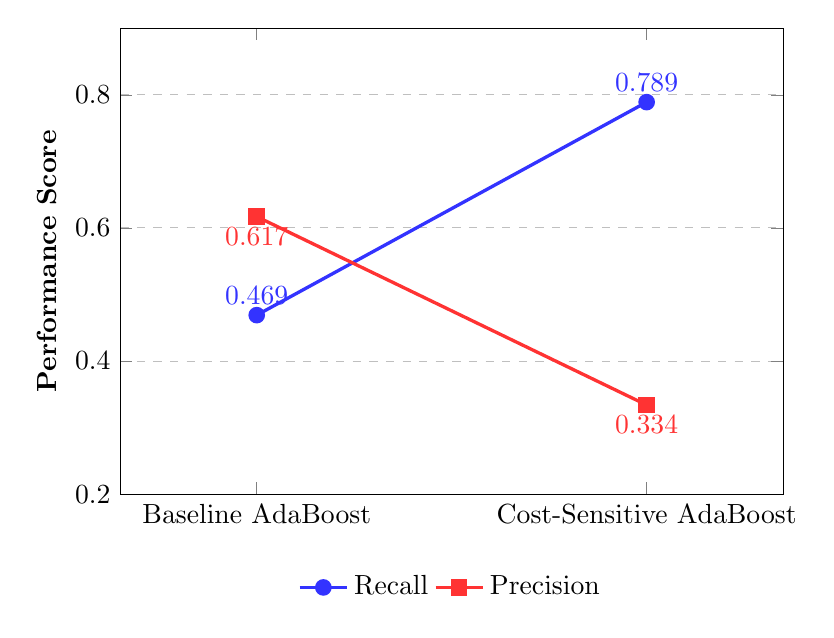
\begin{tikzpicture}
        \begin{axis}[
            width=10cm,       % 圖表寬度
            height=7.5cm,     % 圖表高度
            ymin=0.2, ymax=0.9, % Y軸範圍設定 (因為數值在 0.334 到 0.789 之間)
            ytick={0.2, 0.4, 0.6, 0.8},
            ylabel={\textbf{Performance Score}},
            symbolic x coords={Baseline AdaBoost, Cost-Sensitive AdaBoost},
            xtick=data,
            enlarge x limits=0.35, % 讓 X 軸左右兩側留白，避免資料點貼在邊框上
            ymajorgrids=true,      % 開啟 Y 軸的水平網格線
            grid style=dashed,     % 網格線設為虛線
            legend style={at={(0.5,-0.15)}, anchor=north, legend columns=2, draw=none}, % 將圖例無框放置於圖表正下方
            nodes near coords,     % 自動在資料點旁邊顯示數值
            every node near coord/.append style={font=\bfseries, /pgf/number format/fixed, /pgf/number format/precision=3}
        ]
        
        % 1. 繪製 Recall 折線 (藍色、圓點)
        % 設定數值顯示在點的「上方(above)」，跟著上升趨勢
        \addplot[
            color=blue!80,
            mark=*,
            mark options={scale=1.2},
            very thick,
            nodes near coords align={above} 
        ] coordinates {
            (Baseline AdaBoost, 0.469)
            (Cost-Sensitive AdaBoost, 0.789)
        };
        \addlegendentry{Recall}

        % 2. 繪製 Precision 折線 (紅色、方塊)
        % 設定數值顯示在點的「下方(below)」，跟著下降趨勢，避免與藍線重疊
        \addplot[
            color=red!80,
            mark=square*,
            mark options={scale=1.2},
            very thick,
            nodes near coords align={below} 
        ] coordinates {
            (Baseline AdaBoost, 0.617)
            (Cost-Sensitive AdaBoost, 0.334)
        };
        \addlegendentry{Precision}
        
        \end{axis}
    \end{tikzpicture}
    \caption{Dual-metric line chart illustrating the "death cross" effect in the AdaBoost group. After applying the cost-sensitive mechanism, Recall (blue line) surges dramatically while Precision (red line) experiences a severe collapse, highlighting an extreme trade-off.}
    \label{fig:adaboost_linechart}
\end{figure}

\end{document}